\documentclass[12pt,a4paper]{article}
\usepackage[margin=1in, includeheadfoot]{geometry}

\usepackage[dvipsnames]{xcolor}

\usepackage[dvipsnames]{xcolor}
\usepackage{amsmath}
\usepackage{amssymb}
\usepackage{amsthm}
\usepackage{makeidx}
\usepackage{thmtools}
\usepackage{graphicx}
\usepackage{hyperref}
\usepackage{tikz}
\usepackage{algpseudocode}
\usepackage{multirow}
\usepackage{tcolorbox}

\usetikzlibrary{positioning}

\usepackage{thmtools}
\usepackage[skip=6pt]{parskip}

\usepackage{fancyhdr}
\pagestyle{fancy}

\fancyhead[L]{\textbf{Errata to MPC Course}}
\fancyhead[R]{\thepage}
\fancyfoot{}

\setlength\parindent{0pt}

\hypersetup{
	colorlinks=true,
	linkcolor=RawSienna,
	filecolor=red,  
	citecolor=Aquamarine,    
	urlcolor=blue,
	pdftitle={Errata to MPC Course},
	pdfpagemode=FullScreen,
}

\usepackage[framemethod=tikz]{mdframed}

%\newtcbtheorem[number within=section]{theorem}{Theorem}%
%{colback=RoyalBlue!5,colframe=RoyalBlue!35!black,fonttitle=\bfseries}{th}

\declaretheorem[name=Theorem, numberwithin=section]{theorem}
\declaretheorem[name=Lemma, numberwithin=section]{lemma}
\declaretheorem[name=Inequality, numberwithin=section]{inequality}
\declaretheorem[name=Definition, numberwithin=section]{definition}


\usepackage[english]{babel}
\title{\textbf{Errata to MPC Course}}
\author{Naman Kumar}


\newcommand{\np}{\mathbf{NP}}
\newcommand{\p}{\mathbf{P}}
\newcommand{\ip}{\mathbf{IP}}
\newcommand{\pspace}{\mathbf{PSPACE}}
\newcommand{\am}{\mathbf{AM}}
\newcommand{\ma}{\mathbf{MA}}
\newcommand{\F}{\mathbb{F}}
\newcommand{\E}{\mathbb{E}}
\newcommand{\rel}{\mathcal{R}}
\newcommand{\lang}{\mathcal{L}}
\newcommand{\query}{\mathcal{Q}}
\newcommand{\prover}{\mathcal{P}}
\newcommand{\verifier}{\mathcal{V}}
\newcommand{\decision}{\mathcal{D}}
\newcommand{\simulator}{\mathcal{S}}
\newcommand{\sat}{\mathsf{SAT}}
\newcommand{\ph}{\mathbf{PH}}
\newcommand{\hvzk}{\mathbf{HVZK}}
\newcommand{\zk}{\mathbf{ZK}}
\newcommand{\pzk}{\mathbf{PZK}}
\newcommand{\czk}{\mathbf{CZK}}
\newcommand{\szk}{\mathbf{SZK}}
\newcommand{\pc}{\mathsf{pc}}
\newcommand{\vc}{\mathsf{vc}}
\newcommand{\vr}{\mathsf{vr}}
\newcommand{\poly}{\mathsf{poly}}
\newcommand{\add}{\mathsf{add}}
\newcommand{\mul}{\mathsf{mul}}
\newcommand{\view}{\textsc{view}}
\newcommand{\ideal}{\textsc{ideal}}
\newcommand{\real}{\textsc{real}}
\newcommand{\out}{\textsc{out}}
\newcommand{\bpp}{\mathbf{BPP}}
\newcommand{\rgets}{\xleftarrow{\$}}
\newcommand{\pk}{\mathsf{pk}}
\newcommand{\sk}{\mathsf{sk}}
\newcommand{\secpar}{\lambda}
\newcommand{\gen}{\mathsf{Gen}}
\newcommand{\enc}{\mathsf{Enc}}
\newcommand{\dec}{\mathsf{Dec}}
\newcommand{\func}{\mathcal{F}}
\newcommand{\crs}{\mathsf{crs}}
\newcommand{\KeyGen}{\mathsf{KeyGen}}
\newcommand{\ddh}{\mathbf{DDH}}
\newcommand{\dcr}{\mathbf{DCR}}
\newcommand{\qr}{\mathbf{QR}}
\newcommand{\lwe}{\mathbf{LWE}
}
\newcommand{\lpn}{\mathbf{LPN}}
\newcommand{\cdh}{\mathbf{CDH}}



\newcommand{\rarrow}{\marginpar[\raggedleft\textcolor{red}{$\Longrightarrow$}]{$\Leftarrow$}}

\begin{document}
	\maketitle
	
	\begin{abstract}
		Basic notes on MPC.
	\end{abstract}
	
	\pagebreak
	\tableofcontents
	\reversemarginpar
	
	\pagebreak
	\section{Secure $N$-party Computation}

It's probably worth reiterating some of the formalisms of these definitions with a bit more lucidity, just as a simple reference and as some sort of illumination.

\subsection{Real World Instantiation} In the real world, $N$ parties have inputs $\mathbf{x}=(x_1,\dots,x_n)$, an agreed-upon function $f:(x_1,\dots,x_n)\mapsto(y_1,\dots,y_n)$ and they follow a protocol $\Pi$ which gives them the set of \textit{party outputs} $\out_{\Pi}(\lambda,\mathbf{x}):=(y_1,\dots, y_n)$. Assume that $t$ of these parties are controlled by the adversary; define the \textit{view} $\view_{\Pi,\mathcal{A}}(\lambda, \mathbf{x})$ to be the set of all inputs of corrupted parties, along with messages exchanged that the adversary has sent, received, or eavesdropped-upon.

\begin{definition}[Real World Distribution] The real-world output $\real_{\Pi,\mathcal{A}}(\lambda,\mathbf{x})$ is defined as the tuple
	$$\real_{\Pi,\mathcal{A}}(\lambda,\mathbf{x}):=(\out_{\Pi}(\lambda,\mathbf{x}),\view_{\Pi,\mathcal{A}}(\lambda, \mathbf{x})).$$	
\end{definition}

\subsection{Ideal World Instantiation} In the ideal world, there is no protocol, only a functionality $\mathcal{F}$ which takes in inputs from each party, computes the output $f$, and returns $(f(x_1),\dots,f(x_n))$ to the parties. The output, $\out_{F}(\lambda,\mathbf{x})$ is the same \textbf{--} the output of the parties after the protocol execution \textbf{--} while instead of the \textit{view} (which is, of course, not identical to that of the actual ideal-world `protocol' execution; a protocol could be multi-round), there is the \textit{view of a simulator} (a `fake' adversary which works in the ideal world, but has access to the inputs of the real adversary), which is the output of the simulator on any given execution. 

\begin{definition}[Ideal World Distribution] The ideal-world output $\ideal_{\mathcal{F},\mathcal{S}}(\lambda,\mathbf{x})$ is defined as the tuple
$$\ideal_{\mathcal{F},\mathcal{S}}(\lambda,\mathbf{x}):=(\out_{\mathcal{F}}(\lambda,\mathbf{x}),\view_{\mathcal{F},\mathcal{S}}(\lambda, \mathbf{x})).$$	
\end{definition}

Note that these distributions are \textit{joint} distributions.

\subsection{Secure $N$-Party Protocol}

\begin{definition}[$t$-Privacy of a Protocol]
	An $N$-Party protocol $\Pi$ is considered $t$-private if for any PPT adversary that corrupts $t$ of the parties, there exists a PPT simulator such that
	$$\{\ideal_{\mathcal{F},\mathcal{S}}(\lambda,\mathbf{x})\}\equiv\{\real_{\Pi,\mathcal{A}}(\lambda,\mathbf{x})\}.$$
\end{definition}

\paragraph{Remark.} There's two examples here of the non-privacy of a protocol. One of them is a function which takes no inputs and outputs a random $b\leftarrow\{0,1\}$ to one of the parties, say $P_0$. The protocol in which $P_1$ samples a bit and sends it to $P_0$ is not secure since if $P_1$ is corrupted, the view of the adversary is different; it has the bit $b$ in it. Similarly, if a functionality takes no input and outputs $pq$, $(p+q)$ to the parties, then, again, the protocol in which $P_0$ chooses $p,q$ and sends $p+q$ is insecure since it learns the numbers $p$ and $q$.
	
	\pagebreak
	\section{Containments of $\ip$}
Before we prove the other side of $\ip=\pspace$, we turn our attention to understanding more containments of $\ip$. The techniques developed in this section will be integral in proving that $\pspace\subseteq\ip$ and in showing how IPs are developed for problems which don't have the nice properties of $\mathsf{GNI}$. In particular, we will be proving the following two theorems.

\begin{theorem}
	\label{thm:unsat}
	$\mathsf{UNSAT}\in\ip$. Since $\mathsf{UNSAT}$ is $co\np$-complete, $co\np\subseteq\ip$.
\end{theorem}
\begin{theorem}
	$\#\mathsf{SAT}\in\ip$. Since $\#\mathsf{SAT}$ is $\p^{\#\p}$-complete, $\p^{\#\p}\subseteq\ip$.
\end{theorem}

\subsection{Arithmetization}

We consider \textit{boolean formulae} of the form $\phi(x_1,\dots,x_n)$, which are trees in which
\begin{itemize}
	\item Every leaf node is labelled with a variable $x_i$, and
	\item Every internal node is a logical operator $(\wedge, \vee, \neg).$
\end{itemize}

The goal of the arithmetization procedure is to reduce each boolean formula to a corresponding polynomial, such that $\phi(x_1,\dots,x_n)=p(x_1,\dots,x_n)$. Furthermore, we require $\mathsf{deg}(p)\leq|\phi|$, and that any evaluation of $p$ at a point can be done in $|\phi|$ operations.

This can be accomplished through replacing each variable with the following.
\begin{align*}
	\neg x&\Leftrightarrow 1-x\\
	x_1\wedge x_2&\Leftrightarrow x_1\cdot x_2\\
	x_1\vee x_2&\Leftrightarrow x_1+x_2
\end{align*}

\subsubsection{Application to $\mathsf{UNSAT}$}

Let $\phi$ be a $\mathsf{3CNF}$. Then we have
\begin{align*}
	\phi\in\mathsf{UNSAT}&\implies\sum_{a_1,a_2,\dots,a_n\in\{0,1\}}p(a_1,\dots,a_n)=0\\ \phi\notin\mathsf{UNSAT}&\implies\sum_{a_1,a_2,\dots,a_n\in\{0,1\}}p(a_1,\dots,a_n)>0
\end{align*}

In other words, the sum of the corresponding polynomial over the boolean hypercube is zero if $\phi\in\mathsf{UNSAT}$, since on every input $\phi$ evaluates to $0$, and strictly greater than $0$ if $\phi\notin\mathsf{UNSAT}$, since $\phi$ must have at least one satisfying assignment. Furthermore, this fact remains true over all finite fields of sufficiently large size (in particular, size greater than $2^n3^m$, where $3^m$ is the number of formulae, and $2^n$ is the number of satisfying assignments).

We will now use this fact to obtain an IP for $\mathsf{UNSAT}$.

\subsection{The Sumcheck Protocol}

Sumcheck is a powerful and well-studied protocol first introduced in 1992 \cite{10.1145/146585.146605}. Many improvements to sumcheck have been made over the years, and today it is regularly used in prototype cryptographic systems as an interactive proof system for verifying polynomial addition.

\begin{definition}[Sumcheck.]
	The sumcheck protocol is an IP for verifying that, given $(p,n,H,\gamma,\F)$, where $p$ is a polynomial of degree $n$ that takes $m$ variables, $H$ is any subset of $\F$, and $\gamma\in\F$,
	$$\sum_{\mathbf{x}\in H^m}p(\mathbf{x})=\gamma.$$
	The protocol for sumcheck is given in \ref{fig:3}.
\end{definition}

\begin{figure}[h]
	\begin{mdframed}[
		linecolor=black,
		linewidth=1pt,
		roundcorner=5pt,
		backgroundcolor=white,
		userdefinedwidth=\textwidth,
		]
		\vspace{2mm}
		\begin{enumerate}
			\item $\prover$ calculates the polynomial 
			$$p_1(x)=\sum_{a_2,\dots,a_n\in H}p(x, a_2,\dots,a_n)$$ and sends it to $\verifier$. 
			\item $\verifier$ checks whether $\sum_{a_1\in H}p_1(a_1)=\gamma$. If the check passes, it samples a challenge $w_1\in\F$ and sends it to $\prover$.
			\item $\prover$ calculates $$p_2(x)=\sum_{a_3,\dots,a_n\in H}p(w_1,x, a_3,\dots,a_n)$$ and sends it to $\verifier$.
			\item $\verifier$ checks whether $\sum_{\mathbf{x}\in H^m}p_2(x)=p_1(w_1)$. If the check passes, it samples another challenge $w_2\in\F$ and sends it to the prover.
			\item The protocol proceeds as in the previous two rounds. In the $i^{\text{th}}$ round, $\prover$ calculates $p_i(x)$ and sends it to the verifier, and the verifier checks whether $\sum_{\mathbf{x}\in H^m}p_i(x)=p_{i-1}(w_{i-1}).$
			\item In the last round, $\prover$ sends the polynomial $p_n(x)=p(w_1,\dots,x)$. $\verifier$ samples $w_n$ and checks whether $p_n(w_n)=p(w_1,\dots,w_n)$, and outputs the result.
		\end{enumerate}
		\vspace{2mm}
	\end{mdframed}
	\caption{The Sumcheck Protocol.}
	\label{fig:3}
\end{figure}

\textbf{Note.} It is interesting to see that the verifier's messages in this protocol are all completely \textit{random}. This fact is of independent cryptographic interest, and can be used to make the protocol non-interactive.
\vspace{3mm}

\begin{theorem}
	Sumcheck is a correct IP for the sum of polynomial evaluations over a subset.
\end{theorem}

\begin{proof}
	We begin by checking completeness. Given that $\sum_{\mathbf{x}\in H^m}p(\mathbf{x})=\gamma$, an honest prover can always form the correct polynomials $p_i$ such that any challenge by the verifier is always answered in the affirmative. 
	
	The more difficult check is that of soundness. We will show that given $\sum_{\mathbf{x}\in H^m}p(\mathbf{x})\neq\gamma$, $\verifier$ outputs $1$ with probability
	$$\frac{n\deg(p)}{|\F|}$$
	
	Define $W$ be the event of $\verifier$ accepting, and let $E_i$ be the event that $\tilde{p}_i=p_i$ (where $\tilde{p}_i$ is the polynomial output by a potentially dishonest prover.) We need to place a bound on $\Pr[W]$.
	
	We will begin by showing that for $j\in[n]$,
	$$\Pr[W]\leq\frac{(n-j+1)\deg(p)}{|\F|}+\Pr[W\mid\wedge_{i=j}^n E_i]$$
	
	To show this, we use the Schwartz-Zippel Lemma.
	
	\begin{lemma}[Schwartz-Zippel]
		\label{lem:schwartz-zippel}
		Let $f\in\F[x_1,\dots,x_n]$ be a nonzero multivariate polynomial of degree $d$. Then for any set $S\subseteq\F$, we have
		$$\Pr_{\alpha_i\leftarrow S}[f(\alpha_1,\dots, \alpha_n) = 0]=\frac{d}{|S|}.\qed$$
	\end{lemma}
	
	We proceed by induction. For the base case $j=n, \Pr[W]=\Pr[W\mid E_n]+\Pr[W\mid\overline{E_n}]$.
	$$\Pr[W\mid\overline{E_n}]=\Pr[W\mid\tilde{p}_n(w_n)=p_n(w_n)\mid\tilde{p_n}\neq p_n]\leq\frac{\deg{p_n-\tilde{p}_n}}{|\F|}\leq\frac{\deg(p)}{|\F|}$$
	
	Where the inequality comes from \ref{lem:schwartz-zippel}. For the inductive step,
	\begin{align*}
		\Pr[W]&\leq\frac{(n-j+1)\deg(p)}{|\F|}+\Pr[W\mid\wedge_{i=j}^n E_i]\\
		&\leq\frac{(n-j+1)\deg(p)}{|\F|}+\Pr[W\mid E_{j-1}\wedge\wedge_{i=j}^n E_i]+\Pr[W\mid\overline{E_{j-1}}\wedge\wedge_{i=j}^n E_i]\\
		&\leq\frac{(n-j+1)\deg(p)}{|\F|}+\frac{\deg(p)}{|\F|}+\Pr[W\mid\wedge_{i=j-1}^n E_i]\\
		&\leq\frac{(n-(j-1)+1)\deg(p)}{|\F|}+\Pr[W\mid\wedge_{i=j-1}^n E_i]
	\end{align*}
	It follows that for $j=1$, we have
	$$\Pr[W]\leq\frac{n\deg(p)}{|\F|}+\Pr[W\mid\wedge_{i=1}^nE_i]$$
	But $\Pr[W\mid E_1]=0$, since $\sum_{\alpha\in H}p_1(\alpha)\neq\gamma$. Thus, we can conclude that
	$$\Pr[W]\leq\frac{n\deg(p)}{|\F|}.$$
\end{proof}

\subsection{An IP for $\mathsf{UNSAT}$}

We can obtain an IP for $\mathsf{UNSAT}$ from sumcheck, thereby proving \ref{thm:unsat}. The IP proceeds as follows. Both the prover and the verifier pick a prime $q>2^n3^m$ and work over $\F_q$ (to do this, the $\prover$ sends $\verifier$ a \textit{claimed} prime, which $\verifier$ can verify in polytime since $\mathsf{PRIMES}\in\p$). They then arithmetize $\phi\mapsto p$. Finally, the prover sends the verifier a claimed value of $\sum_{\mathbf{x}\in\{0,1\}}p(\mathbf{x})$, and they run the sumcheck protocol. If $\verifier$ accepts on $\mathbf{x}=\mathbf{0}$, then it outputs $1$, otherwise it outputs $0$.

\subsection{An IP for $\#\mathsf{SAT}$}

The IP for $\#\mathsf{SAT}$ is similar, but unlike $\mathsf{UNSAT}$, we require that we exactly count the number of satisfying assignments. This means that the arithmetization we described in $2.1$ does not immediately work since $x_1+x_2\geq1$, and in particular, $\phi(x_1,\dots, x_n)=0$ implies that $p(x_1,\dots,x_n)=0$, but $\phi(x_1,\dots, x_n)=1$ only implies that $p(x_1,\dots,x_n)>0$. Fortunately, there is a simple fix:
\begin{align*}
	\neg x&\Leftrightarrow 1-x\\
	x_1\wedge x_2&\Leftrightarrow x_1\cdot x_2\\
	x_1\vee x_2&\Leftrightarrow x_1+x_2-xy
\end{align*}

The $-xy$ term in $x_1\vee x_2$ ensures that $x_1\vee x_2\leq 1$, and we can thus adapt the $\mathsf{UNSAT}$ protocol for $\#\mathsf{SAT}$. Note that $q>2^n$ suffices, since $p$ is boolean on boolean inputs.
	
	\pagebreak
	\section{$\pspace\subseteq\ip$}
Using the tools we have developed in the previous section, we are now ready to show the other side of $\ip=\pspace$. Our approach will be nearly identical to our IPs for $\mathsf{UNSAT}$ and $\#\mathsf{SAT}$ \textbf{--} first we identify a $\pspace$-complete problem that deals with boolean formulae, then we arithmetize it, and finally we run a counting IP to decide the arithmetization.

\subsection{Quantized Boolean Formulae}

\begin{definition}[Fully Quantized Boolean Formula]
	A QBF is a logical expression of the form
	$$\sim_1x_1, \sim_2x_2,\dots, \sim_nx_n \phi(x_1,x_2,\dots,x_n)$$
	where $\phi(x_1,\dots,x_n)$ is a CNF, and $\sim_i$ is either $\forall$ or $\exists$ operator.
\end{definition}

Each QBF evaluates to either true or false. In fact, we can view $\np$, $co\np$ and various other complexity through the lens of QBFs:
\begin{align*}
	\np&:=\{\phi\mid\exists x_1,\dots,\exists x_2\phi(x_1,\dots,x_n=1)\}\\
	co\np&:=\{\phi\mid\forall x_1,\dots,\forall x_2\phi(x_1,\dots,x_n=1)\}
\end{align*}

We can further recall that $\ph$ is defined by QBFs in which the quantifiers alternate. The fact that $\ph\subseteq\pspace$ can be easily seen once derive the following result.

\begin{definition}[TQBF]
	$\mathsf{TQBF}$ is the language consisting of 3-CNFs with alternating quantifiers, ie.
	$$\mathsf{TQBF}=\{\phi(x_1,x_2,\dots,x_n)\mid\forall x_1,\exists x_2,\dots\phi(x_1,x_2,\dots,x_n)=1\}$$
\end{definition}

\begin{theorem}
	\label{thm:tqbf}
	$\mathsf{TQBF}$ is $\pspace$-complete.
\end{theorem}

We will look at the proof of \ref{thm:tqbf} in a later section.

\subsection{Arithmetization of $\mathsf{TQBF}$}
Before we can start running an interactive proof over $\mathbf{TQBF}$, we arithmetize it to a polynomial. The inner 3-CNF can simply be arithmetized as the polynomial for $\#\sat$. The transformation for the outer quantifers is more involved, but comes intuitively from the definition.
\begin{itemize}
	\item $\forall$ acts as a conjunction, since $\forall x_i \phi=\phi(x_1,\dots,1,\dots,x_n)\wedge\phi(x_1,\dots,0,\dots,x_n)$.
	\item $\exists$ acts as a disjunction, since $\forall x_i \phi=\phi(x_1,\dots,1,\dots,x_n)\vee\phi(x_1,\dots,0,\dots,x_n)$.
\end{itemize}

Thus, we can arithmetize the quantifiers as
\begin{align*}
	\forall  x_i \phi(x_1,\dots,x_i,\dots,x_n)&\Leftrightarrow p_{\phi}(x_1,\dots,0,\dots,x_n) p_{\phi}(x_1,\dots,1,\dots,x_n)\\
	\exists  x_i \phi(x_1,\dots,x_i,\dots,x_n)&\Leftrightarrow 1-((1-p_{\phi}(x_1,\dots,0,\dots,x_n)) (1-p_{\phi}(x_1,\dots,1,\dots,x_n)))
\end{align*}

We assign symbols to these operations, namely $\prod_{x_i}$ and $\coprod_{x_i}$.

There is a slight problem, however. Since we are multiplying polynomials a total of $2^n$ times (each variable has a quantifier) our final polynomial will contain variables of the form $x^{2^n}$, a calculation the verifier cannot do in polynomial time. However, we notice that $\phi(\mathbf{x})=p(\mathbf{x})\leq 1$. If this is the case, then $x_i^k$ can be replaced by $x_i$ in all fields (including $\F_2$). Thus, we have to add an additional degree quantifier, $\Delta$, which performs the \textit{degree reduction} operation\footnote{It should be clear why $\verifier$ cannot multiply polynomials in polynomial amount of time. It is less apparent, however, why the verifier cannot simply do degree reduction by itself by a simple sift through the monomial expansion. The reason is that the monomial expansion is a particularly inefficient representation of polynomials which takes more than polynomial amount of space in the number of variables. Thus the obvious algorithm is not actually a polytime operation. The `correct' representation of polynomials is in the form of an arithmetic circuit, and degree reduction is not a polynomial-time operation under this representation.}.

Our final arithmetization becomes
$$\forall x_1,\exists x_2,\dots,\phi(\textbf{x})\Leftrightarrow\prod_{x_1}\Delta_{x_1}\coprod_{x_2}\Delta_{x_1}\Delta_{x_2}\dots p_{\phi}(\mathbf{x})$$

\subsection{Shamir's Protocol}

The protocol we now describe was given by Adi Shamir in his original \cite{10.1145/146585.146609} paper. It is a variation of the sumcheck protocol that also allows evaluation of our new quantifier arithmetizations. The protocol is described in \ref{fig:4}. It proceeds for a total of $O(n^2)$ rounds.


\begin{figure}[h]
	\begin{mdframed}[
		linecolor=black,
		linewidth=1pt,
		roundcorner=5pt,
		backgroundcolor=white,
		userdefinedwidth=\textwidth,
		]
		\vspace{2mm}
		\begin{enumerate}
			\item In the $i^{\text{th}}$ step, $\prover$ sends the polynomial $p_i$ to the verifier, which represents the polynomial in the $i^{\text{th}}$ variable with all the later quantifiers applied and all the previous variables substituted by the verifier's random challenges $w_i$.
			\begin{enumerate}
				\item If the quantifier is $\prod/\coprod$, the polynomial is a one-degree polynomial.
				\item If the quantifier is $\Delta$, the polynomial is a $3m$- or $2$- degree polynomial, the polynomial \textit{before} it became the degree-reduced version of the previous round. In the first $n-1$ variable, this is a $2$ degree polynomial since it is the product of two different $1$-degree polynomials. In the last variable, it is the arithmetization itself, which could have up to a $3m$-degree. 
			\end{enumerate}
			\item On receiving this polynomial, the verifier does one of the following:
			\begin{enumerate}
				\item If the $i^{\text{th}}$ quantifier is $\prod$, it checks if $p_i(0)p_i(1)=\gamma_{i-1}=p_{i-1}(w_{i-1})$, the evaluation of the previous step.
				\item If the quantifier is $\coprod$, it checks if $1-(1-p_i(0))(1-p_i(1))=\gamma_{i-1}$.
				\item If the quantifier is $\Delta$, it checks if $p_i(\mathbf{w}_{i-1})=\gamma_{i-1}$, where $\mathbf{w}_i=(w_1,\dots,w_i)$, since the degree-reduced polynomial should have the same evaluation.
			\end{enumerate}
			\item The verifier sends a challenge $w_{i}\leftarrow\F$.
			\item After $O(n^2)$ rounds, the verifier checks if $p(w_1,\dots,w_n)=\gamma_k$.
		\end{enumerate}
		\vspace{2mm}
	\end{mdframed}
	\caption{Shamir's Protocol.}
	\label{fig:4}
\end{figure}

\begin{theorem}
	\label{thm:shamir}
	Shamir's Protocol is a correct IP for $\mathsf{TQBF}$.
\end{theorem}

\begin{proof}
	The full proof can get a bit tedious, but the high-level overview follows from a good understanding of the sumcheck protocol. Completeness is guaranteed from the fact that an honest prover will correctly send the polynomials $p_i$ and finally $p(w_1,\dots,w_n)=\gamma_k$ follows from correctness and definition of the $p_i$.
	
	For soundness, we use similar properties as that of sumcheck, but separate our analysis into two cases:
	
	\begin{itemize}
		\item\underline{Case 1}: The round is a $\prod/\coprod$ round. In this case the prover can't send the correct polynomial $p_i$ since the arithmetized polynomial does not evaluate to a nonzero value, and so $p_i(0)p_i(1)\neq\gamma_{i-1}$. Hence it must send an incorrect polynomial $\tilde{p}_i$ which passes the check. The probability that $\tilde{p}$ passes the verifier's check is $\Pr[\tilde{p}_i(w_i)=p_i(w_i)]\leq\frac{1}{\F}$.
		\item\underline{Case 2}: The round is a $\Delta$ round. In this case the same applies, but the degree of the polynomial is higher, so the error is at most $\frac{3m}{\F}$ or $\frac{2}{\F}$.
	\end{itemize}

	The total soundness error we get is $\frac{1}{\F}(n+\sum_{i=1}^{n-1}2i+3mn)=\frac{3mn+n^2}{\F}$, and if we take $\F$ large enough, the error can get as small as we like.
\end{proof}

We have thus shown an IP for $\mathsf{TQBF}$. To complete our proof, we show that $\mathsf{TQBF}$ is $\pspace$-complete.

\subsection{$\pspace$-completeness of $\mathsf{TQBF}$}

We will now provide a proof of \ref{thm:tqbf}.

\begin{proof}
	First, we see that $\mathsf{TQBF}$ is actually in $\pspace$. To show this, it is enough to notice that evaluating the QBF over all possible inputs along with keeping a polysize tab on whether each quantifier is satisfied is enough. The evaluation of the QBF over all inputs can be easily done in polyspace, since each evaluation can be done in polytime as well.
	
	We now show that $\mathsf{TQBF}$ is $\pspace$-hard. Consider a language $L\in\pspace$. We wish to construct in polytime a polysize QBF $\phi$ such that $x\in L\iff\phi\in\mathsf{TQBF}$. We will use a Turing Machine reduction for this.
	
	First, consider the \textit{configuration graph} $\mathcal{C}_x$ of the computation for $L$ on $x$, which is the graph with nodes corresponding to valid configurations of the TM that computes $L$ and directed edges between valid $1$-step transitions during the evaluation on $x$. Let $C_s$ be the universal start state and $C_a$ be the universal accept state. It follows that
	$$x\in L\iff P(C_s, C_a)\in\mathcal{C}_x$$
	ie, there exists a path between $C_s$ and $C_a$ in $\mathcal{C}_x$. Furthermore, the path length is of less than $2^{O(S(n))}$, since the total number of configurations of that amount. We will recursively define our QBF $\Phi=\Phi_{S(n)}$. We begin by defining
	$$\Phi_i(C,C')=1\iff\exists P(C, C')\in\mathcal{C}_x, |P|\leq 2^i$$ 
	First, $\Phi_1$ is simply the Cook-Levin formula corresponding to a 1-step transition between $C$ and $C'$. This is polysize and contains no quantifiers. Recursively we can then define
	$$\Phi_i(C, C')=\exists C''\Phi_{i-1}(C, C'')\wedge\Phi_{i-1}(C'', C)$$
	The problem is that this effectively doubles the size of the formula, which we can't afford (as it will take more than polynomial the amount of space). To offset this, we introduce new variables $D_1$ and $D_2$ such that 
	$$\Phi_i(C, C')=\exists C''\forall D_1, D_2 (D_1=C\wedge D_2=C'')\vee (D_1=C''\wedge D_2=C)\implies \Phi_{i-1}(D_1, D_2)$$
	It is worth looking at what is actually happening here. The two new variables we have introduced sift over all the vertices and check whether there exists some $C''$ for which this works using just a single evaluation of $\Phi_{i-1}$. Parsed, this means that for whatever $D_1$ and $D_2$ that are taken, if even one of the two possible valuations is satisfied, it will follow that $\Phi_{i-1}(D_1, D_2)$ will be true. The `implies' function can be encoded as a formula with just a polynomial overhead. Thus there is only a polynomial size jump at each step, and we have
	$$\Phi_i=\Phi_{i-1}+\mathsf{poly}(S(n)$$
	It follows that $\Phi_{S(n)}$ is polysize. Thus, $\mathsf{TQBF}$ is $\pspace$-complete.
\end{proof}

Theorems \ref{thm:tqbf} and \ref{thm:shamir} together imply that $\pspace\subseteq\ip$. The other direction was previously shown. It follows that the class of languages decidable by $\ip$ is exactly equal to the class decidable by $\pspace$, which, according to conventional belief, gives a considerable amount of power over base $\np$.

\begin{theorem}
	\label{thm:ip=pspace}
	$\ip=\pspace$.
\end{theorem}
\begin{proof}
	Follows from \ref{thm:ipsubsetpspace}, \ref{thm:tqbf} and \ref{thm:shamir}.
\end{proof}

	\pagebreak
	\section{OT Extension}

As we have seen, it is possible to perform OT of strings of long length using OT for strings of shorter length and a PRG. We will now answer the question of whether it's possible to perform a greater \textit{number} of OTs using a fewer number of OTs.

\subsection{IKNP OT Extension} 

In this section we will describe the IKNP OT Extension protocol from \cite{iknp}. The protocol works by extending $\secpar$ pairs of $m$-bit OT to $m$ pairs of $\ell$-bit OT. A full description is below. We note by $\mathbf{OT}^{a}_{b}$ an $a$-pairs $b$-bit OT functionality.

\begin{figure}[h]
	\begin{mdframed}[
		linecolor=black,
		linewidth=1pt,
		roundcorner=5pt,
		backgroundcolor=white,
		userdefinedwidth=\textwidth,
		]
		\vspace{2mm}
		\textbf{Parameters:} The Sender holds $m$ pairs of $\ell$-bit strings $\{(m_{i,b})\}$. The receiver holds $m$ selection bits $r=(r_1,\dots, r_m)$. $H:[m]\times\{0,1\}^{\secpar}\rightarrow\{0,1\}^\ell$ is a random oracle.\\

		\textbf{Protocol:}		 
		\begin{itemize}
			\item Sender selects $s\rgets\{0,1\}^\secpar$ and sends it to $\mathbf{OT}^{\secpar}_{m}$ (as the receiver).
			\item Receiver selects a random matrix
			$$T=
			\begin{pmatrix}
				T_1 & T_2 & \hdots & T_\secpar
			\end{pmatrix}_{m\times \secpar}=\begin{pmatrix}
			T^1 \\ T^2 \\ \vdots \\ T^m
		\end{pmatrix}_{m\times \secpar}$$ and sends the inputs $\{(T_i, r\oplus T_i)\}_{i\in[\secpar]}$ to $\mathbf{OT}^{\secpar}_{m}$ (as the sender).
			\item Denote by $Q$ the matrix received by the sender, which is
			$$Q=
			\begin{pmatrix}
				Q_1 & Q_2 & \hdots & Q_\secpar
			\end{pmatrix}_{m\times \secpar} = \begin{pmatrix}
			Q^1 \\ Q^2 \\ \vdots \\ Q^m
		\end{pmatrix}_{m\times \secpar}$$
		\item Sender sends 
		$$(y_{j,0}, y_{j,1})=(x_{j,0}\oplus H(j,Q^j), x_{j,1}\oplus H(j, Q^j\oplus s)).$$
		\item For each $1\leq j\leq m$, receiver outputs $y_{j, r_j}\oplus H(j, T^j)$.
		\end{itemize}
		\vspace{2mm}
	\end{mdframed}
	\caption{The IKNP OT Extension Protocol.}
	\label{fig:IKNP}
\end{figure}

\paragraph{Correctness.} We will now see why this protocol works. Consider $r_i = 0$ for some $i$. It follows that $(r_i)_{j\in[\lambda]}\oplus T^i = T^i$, and so $T^i=Q^i$ (regardless of whatever $s$ was). It immediately follows that $H(j, T^j) = H(j, Q^j)$.

On the other hand, if $r_i = 1$, then $Q^i = (s \cdot r)\oplus T^j =s\oplus  T^j$. Correctness follows similarly.

\paragraph{Discussion.} The protocol provides perfect security against a semi-honest (even malicious) sender and statistical security against a semi-honest receiver. The protocol is instantiated with a random oracle, but can be instantiated with a weaker primitive called a \textit{correlation-robust hash function}.

\begin{definition}[Correlation Robustness]
	An efficiently computable function $h:\{0,1\}^{*}\rightarrow \{0,1\}$ is said to be \textit{correlation robust} if for any polynomial $q$ and PPT adversary $\mathcal{A}$ there exists a negligible function $\epsilon(\cdot)$ such that
	$$|\Pr[\mathcal{A}(t_1,\dots,t_m, h(t_1\oplus s), \dots, h(t_m\oplus s))=1]-\Pr[\mathcal{A}(U_{(t+1)m})=1]|\leq\epsilon(\secpar)$$
	where $m\leq q(\secpar)$ and $|C|\leq p(\secpar)$. The probability is taken over random and independent choices of $s, t_i\rgets\{0,1\}^\secpar$ for $i\in[m]$.
\end{definition}

The authors also modify the scheme to achieve full security against a malicious receiver through a cut-and-choose mechanism, in which a the receiver and the sender execute $k$ instances of the (committed) protocol in parallel and the sender randomly checks whether a certain number of instances were correctly performed (and aborts otherwise).

\paragraph{Parameters.} The above protocol is secure as long as $m=2^{o(\secpar)}$. Note that if, say, $m = 2^\secpar$, then the security of the correlation-robust hash function breaks down since this allows a `repeat', i.e. $H(j, Q^j\oplus s)$ will be called twice for some value of $j$. We will see the impossibility of $2^{\Omega(\secpar)}$-pairs OT extension in Minicrypt along with other impossibility results below. This concludes that the protocol is asymptotically optimal.

\paragraph{Improvements.} \cite{vole} achieves $n$ pairs using $\log n$ OTs and the (computational) LPN (Learning Parity with Noise) assumption. \cite{softspokenot} presents a practical improvement on the protocol.

\subsection{Feasibility of OT Extension}

The protocol of \cite{iknp} is not the only OT Extension protocol. Before this, \cite{beaver1996correlated} showed that $k$ OTs can be extended to $k^c$ OTs making a non-black box use of a one way function. The protocol of \cite{iknp} can gain up to superpolynomial OTs with a black-box use of an OWF, but makes use of a Random Oracle.

\textbf{Open Problem.} Is there a protocol for (subexponential) OT extension that makes black-box use of a One Way Function without a random oracle?

\cite{lindell2013feasibility} study the feasibility of OT Extension, and prove the following results.

\begin{theorem}[Information-Theoretic OT Extension]
	If there exists an OT extension protocol from $n$ to $n+1$ (with security in the presence of static semi-honest adversaries), then there exist one-way functions.
\end{theorem}

This proves that OT cannot be extended information-theoretically. Note that while the protocol of \cite{iknp} does not make explicit use of an OWF, it does use a random oracle (which implies OT extension).

\begin{theorem}[Adaptively Secure OT Extension]
	If there exists an OT extension protocol from $n$ to $n+1$ that is secure in the presence of adaptive semi-honest adversaries, then there exists an oblivious transfer protocol that is secure in the presence of static semi-honest adversaries.
\end{theorem}

This proves that any adaptive OT extension protocol involves constructing statically secure OT extension from scratch. The problem of constructing adaptively secure OT extension was solved in \cite{byali2017fast}, though their protocol uses public-key cryptography.

\begin{theorem}[Extending Logarithmic OTs]
	If there exists an OT extension protocol from $f(n)=O(\log n)$ to $f(n)+1$ that is secure in the presence of static malicious adversaries, then there exists an OT protocol that is secure in the presence of static malicious adversaries.
\end{theorem}

This proves that any OT extension protocol that have exponential extension must make use of an exponential number of OTs itself.
	
	\pagebreak
	\section{The GMW Protocol}
	
	\pagebreak
	\section{Delegating Computation and the GKR Protocol (Incomplete)}

Until now we have considered interactive proofs with a polynomial time verifier. While the formal definition of IPs allows the prover to have unbounded computational power, we often consider situations in which the honest prover also works efficiently.

Suppose we are given a boolean formula $\phi=\phi(x_1,\dots,x_n)$. Then,
\begin{itemize}
	\item in the sumcheck protocol for $\#\mathsf{SAT}$, the prover takes time $\Omega(2^n|\phi|)$, since it has to sum over all possible values of $(x_1,\dots,x_n)$.
	\item in Shamir's protocol for $\mathsf{TQBF}$, the prover similarly has to take time $\Omega(2^n|\phi|)$.
\end{itemize}

These times are too high to be practically useful for computation. Suppose we have a machine $M$ that runs in time $T$ and in space $S$. Then, we can reduce the language $L_m=\{x:M(x)=1\}$ to a $\mathsf{TQBF}$ instance $\phi(x_1,\dots,x_n)$, where $$n\geq \log{T}\cdot S$$ Even if both $T,S\in\poly(n)$, it follows that the prover time is $\Omega(2^n)=\Omega(T^S)=n^{\omega(1)}$.

\subsection{Doubly-Efficient Interactive Proofs}

\begin{definition}[Doubly-Efficient Interactive Proof]
	A deIP is an interactive proof in which the prover is additionally constrained to run in polynomial time.
\end{definition}

Intuitively, deIPs are interactive proofs which are `computationally useful,' ie. can be used to delegate computation. These are particularly useful when the verifier requires less resources to run than calculating the proof itself -- for instance, instead of performing a heavy $O(n^6)$ algorithm, the verifier can delegate the task to the prover and simply check the solution using only $O(n)$ or $O(n\log n)$ time. In special cases, the prover may even need to run for time sublinear in the problem length.

We now give a first characterization of $\mathbf{deIP}$.

\begin{theorem}
	$\mathbf{deIP}\subseteq\mathbf{BPP}$.
	\label{thm:deip}
\end{theorem}
\begin{proof}
	The probabilistic algorithm simply simulates the interaction between prover and verifier, which it can do in polynomial time and using the verifier's randomness.
\end{proof}

\subsection{Delegation for Bounded-Depth Circuits}

\begin{definition}[$S$-Space Uniform Circuit Family]
	A circuit family $\mathcal{C}_i=\{C\}_{i\in\mathbb{N}}$ is $S$-space uniform if there exists a machine $M$ such that $M(1^n)=C_n$ and $M$ runs in space $O(S(n))$.
\end{definition}

We now see a theorem that relates $\ip$ and languages decidable by circuits.

\begin{theorem}
	Suppose that $L$ is decidable by an $O(\log S)$-space uniform circuit family of size $S$ and depth $D$. Then $L$ has a public coin IP such that
	\begin{itemize}
		\item the prover time is $\poly(S)$,
		\item the verifier time is $(n+D)\cdot\mathsf{polylog}(S)$ and space is $O(\log S)$,
		\item the total communication is $D\cdot\mathsf{polylog}(S)$.
	\end{itemize}
\end{theorem}

The proof of this theorem is long and technical. We will see only the bare-bones protocol, in which the verifier has query access to the circuit's topology. We will thus not need to discuss uniformity.

The protocol we will discuss is called the GKR protocol and is highly efficient in practice. \cite{10.1145/2699436} was introduced by Goldwasser, Kalai and Rothblum in 2008 and uses ideas of arithmetization and sumcheck. Furthermore, GKR can be modified so that the prover runs in linear time, and the verifier can in fact verify the computation using time sublinear in the size of the circuit.

GKR is also interesting in terms of providing an IP for the circuit complexity class $\mathbf{NC}$. Using GKR yields a polytime prover and a linear time verifier.

\subsubsection{Layered Arithmetic Circuits}

\begin{definition}[Layered Arithmetic Circuit]
	An arithmetic circuit $C:\F^n\rightarrow\F$ of size $S$, depth $D$ and fan-in $2$ arranged in $D+1$ layers.
\end{definition}

\begin{figure}[h]
	\begin{center}
		{\renewcommand{\arraystretch}{1.2}%
		\begin{tabular}{ c c c }
			\hline
			\multirow{2}{6em}{Layer $0$} & \multirow{2}{6em}{$V_0\in\F$} & \\
			&&\\
			\hline
			\multirow{2}{6em}{Layer $1$} & \multirow{2}{6em}{$V_1:S\rightarrow\F$} & $\add_1:[S]^3\rightarrow\{0,1\}$ \\ 
			& & $\mul_1:[S]^3\rightarrow\{0,1\}$ \\
			\hline
			\multirow{2}{6em}{Layer $2$} & \multirow{2}{6em}{$V_2:S\rightarrow\F$} & $\add_2:[S]^3\rightarrow\{0,1\}$ \\ 
			& & $\mul_2:[S]^3\rightarrow\{0,1\}$ \\
			\hline
			\vdots & \vdots & \vdots \\
			\hline
			\multirow{2}{6em}{Layer $D-1$} & \multirow{2}{6em}{$V_{D-1}:S\rightarrow\F$} & $\add_{D-1}:[S]^3\rightarrow\{0,1\}$ \\ 
			& & $\mul_{D-1}:[S]^3\rightarrow\{0,1\}$ \\ 
			\hline
			\multirow{2}{6em}{Layer $D$} & \multirow{2}{6em}{$V_D:S\rightarrow\F$} & $\add_D:[S]\times [n]^2\rightarrow\{0,1\}$ \\ 
			& & $\mul_D:[S]\times[n]^2\rightarrow\{0,1\}$ \\
			\hline
		\end{tabular}
	}
	\end{center}
	\caption{A Layered Circuit.}
	\label{fig:layeredcircuit}
\end{figure}

Figure \ref{fig:layeredcircuit} gives a functional representation of a layered circuit. At each level are gates, which contain either $+$ or $\times$ and represent the sum or product of the input wires into the gate. We can additionally define two functions $\add_i$ and $\mul_i$.
\begin{align*}
	\add_i(g_j,w_k,w_l)=
	\begin{cases}
		1&\text{if $g_i$ is a $+$ gate with input wires from nodes $w_k$ and $w_l$,}\\
		0&\text{otherwise.}
	\end{cases}
\end{align*}
\begin{align*}
	\mul_i(g_j,w_k,w_l)=
	\begin{cases}
		1&\text{if $g_i$ is a $\times$ gate with input wires from nodes $w_k$ and $w_l$,}\\
		0&\text{otherwise.}
	\end{cases}
\end{align*}

$\add$ and $\mul$ are called \textit{wiring predicates}. For notational simplicity, we assume that $C$ has only one kind of gate, $g:\F^n\rightarrow F$.

\begin{figure}[h]
	\centering
	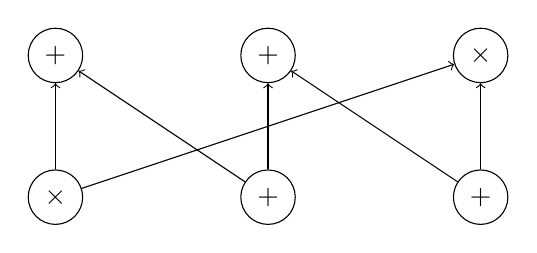
\begin{tikzpicture}  
		[scale=.9,auto=center,every node/.style={circle,draw}] % here, node/.style is the style pre-defined, that will be the default layout of all the nodes. You can also create different forms for different nodes.  
		
		\node (a1) at (0,1) {$+$};  
		\node (a2) at (-3,1)  {$+$}; 
		\node (a3) at (3,1)  {$\times$};  
		\node (a4) at (0,-1) {$+$};  
		\node (a5) at (-3,-1)  {$\times$};  
		\node (a6) at (3,-1)  {$+$};   
		
		\draw [<-] (a1) -- (a4);
		\draw [<-] (a1) -- (a6);
		\draw [<-] (a2) -- (a5);
		\draw [<-] (a2) -- (a4);
		\draw [<-] (a3) -- (a5);
		\draw [<-] (a3) -- (a6);
		
	\end{tikzpicture}  
	\caption{Two Layers of a Circuit.}
\end{figure}

\subsubsection{Low-Degree Extensions}

\begin{definition}[Polynomial Extension]
	Let $H\subseteq\F$ be a domain and $f:H\rightarrow\F$ be a function. Then a polynomial $p\in\F[x]$ is called an extension of $f$ if $p|_H=f$.
\end{definition}

We are interested in low-degree extensions, in which the polynomial has a low degree. The lowest degree (or minimal) extension is the extension obtained through Lagrange Interpolation: the degree is $<|H|$, and can be calculated as
$$p(x)=\sum_{\alpha\in H}f(\alpha)\left[\prod_{\beta\in H\setminus\{\alpha\}}\left(\frac{x-\beta}{\alpha-\beta}\right)\right]$$

The term in the square braces is called the Lagrange polynomial, and we represent it as $L_{\alpha,H}(x)$. We can easily extend this to the multivariate case. It follows that
\begin{itemize}
	\item $p\in\F[x_1,\dots,x_n]$ extends $f:H^n\rightarrow\F$ if $p|_{H^n}=f$.
	\item the extension of minimum degree has individual degree $<|H|$ and equals
	 $$p(x_1,\dots,x_n)=\sum_{\alpha_1,\dots,\alpha_n\in H}f(\alpha_1,\dots,\alpha_n)\left(\prod_{\alpha_i}L_{\alpha_i,H}\right)$$
	 where the product of the lagrange polynomials is the multivariate lagrange polynomial $L_{\alpha_1\dots,\alpha_n, H^n}$.
\end{itemize}

\subsubsection{Layer Arithmetization}


	
	\pagebreak
	\appendix
	
	\pagebreak
	\section{List of Assumptions}

We provide here a lookup table for a list of common assumptions.

\subsection{Assumptions Based on Discrete-Log}

\subsection{Assumptions based on Reciprocity}

\subsection{Assumptions based on Coding}

\subsection{Assumptions based on Lattices}
	
	\pagebreak
	\bibliographystyle{alpha}
	\bibliography{references}
	
\end{document}